\documentclass[times, utf8, zavrsni, numeric]{fer}
\usepackage{booktabs}

\begin{document}

% TODO: Navedite broj rada.
\thesisnumber{6742}

% TODO: Navedite naslov rada.
\title{Sažimanje teksta zasnovano na modelima dubokog učenja}

% TODO: Navedite vaše ime i prezime.
\author{Petar Mihaljević}

% \maketitle

% Ispis stranice s napomenom o umetanju izvornika rada. Uklonite naredbu \izvornik ako želite izbaciti tu stranicu.
% \izvornik

% Dodavanje zahvale ili prazne stranice. Ako ne želite dodati zahvalu, naredbu ostavite radi prazne stranice.
\zahvala{}

\tableofcontents

\chapter{Uvod}
Sažimanje teksta je grana strojnog učenja (obrade prirodnog jezika) koja se bavi kraćenjem dugačkog teksta. Svrha je stvoriti povezan i tečan sažetak koji se sastoji samo od najvažnijih informacija iz originalnog teksta.
U obradi prirodnog jezika, postoje dva glavna načina sažimanja teksta: ekstraktivno i apstraktivno.
Ekstraktivno sažimanje teksta se temelji na izvlačenju ključnih izraza iz izvornog teksta koji se na kraju spajaju u sažetak. Ekstrakcija se vrši na temelju definirane metrike bez mijenjanja izvornog teksta.
Apstraktivno sažimanje teksta uključuje parafraziranje i kraćenje dijelova izvornog teksta. To znači da se izvorni tekst mijenja, čime se mogu izbjeći gramatičke pogreške koje uobičajeno nastaju ekstraktivnim sažimanjem teksta.
Algoritmi apstraktivnog sažimanja teksta stvaraju nove fraze i rečenice i pokušavaju njima prenijeti glavnu ideju izvornog teksta, upravo kako to rade i ljudi kada parafraziraju neki tekst.
Sažimanje teksta se uobičajeno tretira kao nadzirano strojno učenje gdje se budući rezultati predviđaju na temelju pruženih podataka: ulaz i željeni izlaz.
\par
U završnom radu programski je ostvarena desktop aplikacija koristeći Tkinter u Pythonu.
Ta aplikacija služi za sažimanje teksta pri čemu su omogućena oba gore navedena načina sažimanja teksta.
Za ekstraktivno sažimanje teksta korištene su knjižnice kao što su Gensim, SpaCy i Sumy, a za apstraktivno sažimanje teksta dizajnirana je i istrenirana vlastita mreža koja sažima kraće recenzije.
Aplikacija nudi različite mogućnosti zadavanja izvornog teksta, recimo odabirom tekstualne datoteke, utipkavanjem teksta ili zadavanjem URL-a.
\par
Ostatak rada organiziran je na sljedeći način: u 2. poglavlju dat je pregled tehnika sažimanja teksta u obradi prirodnog jezika,
u 3. poglavlju opisana je struktura programskog rješenja ove aplikacije,
u 4. poglavlju dolazi opis problema i programsko ostvarenje mreže za apstrakcijsko sažimanje teksta koja je korištena u aplikaciji,
u 5. poglavlju nalazi se opis postupka vrednovanja mreže te je
u 6. poglavlju iznesen zaključak ovoga rada.

\chapter{Tehnike sažimanja teksta u obradi prirodnog jezika}
\section{Uvod}
Cilj automatskog sustava za sažimanje teksta jest generirati sažetak, odnosno skraćeni oblik dokumenta koji sadrži više važnih rečenica odabranih iz tog dokumenta.
Takav sažetak trebao bi se sastojati od najrelevantnijih informacija u dokumentu, a istodobno bi trebao zauzeti bitno manje prostora od originalnog teksta.
Razmatraju se četiri glavna problema: pokrivenost informacija, informacijski značaj, redundancija u informacijama i kohezija u tekstu.
Trenutno su razvijena dva glavna pristupa u sažimanju teksta koji se mogu svrstati u ekstrakcijsko i apstrakcijsko sažimanje teksta.
Tehnika ekstrakcijskog sažimanja teksta sastoji se od ekstrakcija važnih rečenica iz izvornog dokumenta i predstavljanja tih rečenica u istom redoslijedu kao u izvornom dokumentu.
Važnost rečenica određuje se težinom svake rečenice temeljene na statističkim i jezičnim obilježjima.
Tehnika apstrakcijskog sažimanja teksta sastoji se od razumijevanja glavnih pojmova u izvornom dokumentu i prikazivanja tih pojmova na kraći način.
To zahtijeva ljudsko znanje, statističke metode i jezične metode.
Osim ta dva glavna pristupa postoje i novije metode sažimanja teksta kao što su teorija grafova, latentna semantička analiza (engl. latent semantic analysis), neizrazita logika (engl. fuzzy logic) i druge metode i tehnike.
\section{Vrste sažimanja teksta}
\subsection{Ekstrakcijsko sažimanje dokumenta}
Ekstrakcijski sažetak dokumenta generira se odabirom više relevantnih rečenica iz izvornog dokumenta (\citet{article1}). Duljina sažetka ovisi o stopi kompresije.
Postoji funkcija koja ocjenjuje rečenice iz izvornog dokumenta i rangira ih prema određenoj metrici. Visoko rangirane rečenice se odabiru pri generiranju sažetka. Broj rečenica koji će biti odabran ovisi o stopi kompresije.
Ova metoda je relativno jednostavna i robusna.
Pri generiranju sažetka ne stvaraju se novi izrazi niti rečenice, već se sav sadržaj uzima iz izvornog dokumenta.
\subsection{Apstrakcijsko sažimanje dokumenta}
Za razliku od ekstrakcijskog sažetka, apstrakcijski sažetak uključuje riječi i rečenice različite od onih koje se pojavljuju u izvornom dokumentu.
Apstrakcijski sažetak se sastoji od ideja ili koncepata iz izvornog dokumenta, ali oni se tumače i prikazuju u različitom obliku - parafraziraju se (\citet{article1}).
S obzirom na to da je ovdje potrebna opsežna obrada prirodnog jezika, apstrakcijsko sažimanje teksta je znatno složenije od ekstrakcijskog sažimanja teksta.
Zbog manje složenosti ekstrakcijski sažetak je postao popularniji od apstrakcijskog sažetka.
\subsection{Sažetak jednog dokumenta i sažetak više dokumenata}
Tehnike sažimanja teksta mogu se podijeliti s obzirom na broj dokumenata koji one sažimaju.
Sažetak jednog dokumenta generira se na temelju sadržaja jednog dokumenta, dok se u sažetku više dokumenata koriste mnogi dokumenti za generiranje sažetka.
Sažetak većeg broja dokumenata nije samo jednostavno proširenje algoritma za sažimanje jednog dokumenta jer se pojavljuju dodatni problemi, a jedan od najvećih je redundancija.
Istražuju se različite metode za smanjenje redundancije u sažetku više dokumenata, a najpoznatija među njima je metoda maksimalne marginalne važnosti (eng. MMR method, maximal marginal relevance).
\subsection{Generički sažetak i sažetak usmjeren na upit}
Sažimanje teksta se može podijeliti i na generički sažetak ili sažetak usmjeren na upit.
Sažeci usmjereni na teme ili usredotočeni na korisnike druga su imena za sažetke usmjerene na upit.
Takav sažetak uključuje sadržaj povezan s upitom, dok opći smisao podataka koji se nalaze u dokumentu čini generički sažetak.
\subsection{Nadzirano strojno učenje ili nenadzirano strojno učenje}
Sažimanje teksta može se raditi kao nadzirano strojno učenje ili kao nenadzirano strojno učenje.
Podaci za treniranje potrebni su kod nadziranog strojnog učenja za odabir važnog sadržaja iz dokumenata.
Potrebna je velika količina označenih podataka za tehnike nadziranog strojnog učenja.
Rečenice koje pripadaju sažetku nazivaju se pozitivni uzorci, a rečenice koje nisu sadržane u sažetku nazivaju se negativni uzorci.
Za klasifikaciju rečenica koriste se metode klasifikacije kao što su SVM (eng. support vector machine) i neuronske mreže (\citet{article1}).
\par
Nenadzirano strojno učenje ne zahtijeva nikakve podatke za treniranje. Ovdje se generira sažetak pristupanjem samo odabranim dokumentima.
Ovaj način je prikladan za sve novo promatrane podatke bez ikakvih naprednih modifikacija.
Ovdje se primjenjuju heuristička pravila za izdvajanje relevantnih rečenica i generiranje sažetka.
Tehnika koja se koristi u sustavima bez nadzora je klasteriranje.
\subsection{Indikativni, informativni i kritički ocjenjivački sažetci}
Indikativni sažetci govore o čemu se radi u dokumentu. Oni daju informacije o temi dokumenta.
Informativni sažetci daju cjelokupnu informaciju u razrađenom obliku.
Kritički ocjenjivački sažetak se sastoji od pogleda autora o određenoj temi i sadrži mišljenja, recenzije, preporuke, povratne informacije i slično.
\subsection{Višejezični, jednojezični i jezično neovisni sažeci}
Na temelju jezika sažetci se mogu podijeliti na višejezične, jednojezične i jezično neovisne sažetke.
Ako je jezik izvornog dokumenta i sažetka isti, onda se radi o jednojezičnom sustavu sažimanja.
Kada je izvorni dokument na više jezika, a sažetak se također generira na tim jezicima, onda se radi o višejezičnom sustavu sažimanja.
Ako je izvorni dokument recimo na engleskom jeziku, a sažetak na bilo kojem drugom jeziku osim engleskog, tada je to sustav neovisan o jeziku.
\subsection{Sažimanje teksta na webu}
Tehnike sažimanja teksta na webu komprimiraju važne informacije prisutne na web stranicama.
\subsection{Sažimanje teksta na temelju e-pošte}
Sažimanje teksta na temelju e-pošte je vrsta sažetka u kojem su sažeti e-mail razgovori.
U svijetu poslovanja, sažetak e-pošte može se koristiti kao korporativna memorija gdje sažetci sadrže sve poslovne odluke donesene u prošlosti.
\subsection{Personalizirani sažetci}
Personalizirani sažetci sadrže konkretne informacije koje korisnik želi imati.
Takvi (personalizirani) sustavi nakon određivanja korisničkih profila odabiru bitan sadržaj za izradu sažetka.
Ovdje spadaju i ažurirani sažetci te sažetci na temelju osjećaja.
U ažuriranim sažetcima smatra se da potrošači imaju osnovne informacije o temi i zahtijevaju samo aktualna ažuriranja.
Sažetci na temelju osjećaja se koriste na društvenim mrežama, forumima, blogovima i slično.
\subsection{Ostale vrste sažetaka}
Sažimanje teksta i analiza sentimenta zajedno čine ispitivanje mišljenja i služe za generiranje takvih vrsta sažetaka.
U takvim sažetcima mišljenja se inicijalno otkrivaju i klasificiraju na temelju subjektivnosti, a zatim na temelju polariteta (pozitivno, negativno ili neutralno).
\par
Sažetci anketiranja daju pregled određene teme ili entiteta.
Sažetci anketiranja, biografski sažeci i članci s Wikipedije spadaju u ovu kategoriju.

\begin{table}[htb]
\caption{Vrste sažimanja teksta (\citet{article1})}
\label{tbl:vst}
\centering
\begin{tabular}{l|l} \hline
Vrste sažimanja teksta & Faktori \\ \hline
Sažimanje jednog ili više dokumenata & Broj dokumenata \\
Ekstrakcijsko ili apstrakcijsko & Izlaz u ekstrakcijskom ili apstrakcijskom obliku \\
Generičko i upitno & Namjena, općenito ili upitno povezani podaci \\
Nadgledano i nenadgledano & Dostupnost trening podataka \\
Jednojezično, višejezično i neovisno o jeziku & Jezik \\
Web sažimanje & Za sažimanje teksta na web stranicama \\
E-mail & Za sažimanje e-mail poruka \\
Osobna & Informacije specifične za osobne namjene \\
Ažuriranja & Tekuća ažuriranja zahtijevanih tema \\
Mišljenja i stavovi & Detektiranje stavova i mišljenja \\
Ankete & Važne činjenice o različitim entitetima\\ \hline
\end{tabular}
\end{table}

\section{Ekstrakcijski pristupi za generiranje sažetaka}
\subsection{Statistički utemeljeni pristupi}
Statistički utemeljeni pristupi se oslanjaju na statističke značajke prilikom odabira važnih rečenica za sažetak.
Ove tehnike su jezično neovisne. Ne zahtijevaju dodatno jezično znanje niti složenu jezičnu obradu.
Također, zahtijevaju manje procesorske snage i kapaciteta radne memorije računala od apstrakcijskog sažimanja teksta.
Neke od statističkih značajki su položaj rečenice, pozitivna ključna riječ (na temelju frekvencije pojavljivanja), negativna ključna riječ (na temelju frekvencije pojavljivanja), središnje rečenice (odnosno sličnost s drugim rečenicama), sličnost rečenice s naslovom, relativna duljina rečenice, prisutnost numeričkih podataka u rečenici, prisutnost vlastite imenice u rečenici i slično.
Za svaku rečenicu iz izvornog dokumenta računaju se statističke značajke te se na temelju tih rezultata rečenice rangiraju.
Svaka od gore navedenih značajki dodjeljuje težinu riječima. Na temelju tih težina bodovi se dodjeljuju rečenicama.
Visoko rangirane rečenice odabiru se za generiranje sažetka.
\subsection{Tematski utemeljeni pristupi}
Tema predstavlja o čemu se radi u dokumentu. 
Struktura teme određena je tematskim pojmovima koje predstavljaju događaji koji se često javljaju u zbirci dokumenata.
Teme se mogu prikazati na pet različitih načina:
\begin{enumerate}
  \item Oznake teme: sugeriraju da je potrebna zbirka pojmova za izražavanje teme dokumenta.
  \item Poboljšane oznake tema: Isto kao za oznaku teme, s tim da su važni odnosi otkriveni između dva tematska pojma.
  \item Tematske oznake: Dokumenti se prvo segmentiraju pomoću algoritma. Tada se teme dodjeljuju nekim oznakama kako bi ih kasnije mogli svrstati.
  \item Modeliranje strukture sadržaja dokumenata: tekstovi koje proizvodi određeni model sadržaja opisuju određenu temu.
  \item Predlošci: ovdje su identificirani određeni entiteti ili činjenice.
\end{enumerate}
\subsection{Pristupi utemeljeni na grafovima}
Čvorovi grafa predstavljaju tekstualne elemente (riječi ili rečenice). Čvorovi su povezani bridovima u jedni cjelinu koja predstavlja tekst.
LexRank je preporučeni sustav sažetka za više dokumenata u kojima su prikazane odabrane rečenice na grafu za koje se očekuje da su dio sažetka.
Ako je sličnost između dvije rečenice iznad određenog ograničenja, onda među njima postoji veza u grafu.
Nakon što se napravi mreža, sustav odabire važne rečenice tako da izvrši slučajni hod po grafu.
\subsection{Pristupi utemeljeni na diskursu}
Ovaj se pristup koristi u lingvističkim tehnikama za automatsko sažimanje teksta.
Ovim postupkom se otkrivaju odnosi diskursa u tekstu. Odnosi s diskursom predstavljaju veze između rečenica i dijelova u tekstu.
U računalnoj lingvističkoj domeni je predložena teorija retoričke strukture (eng. rhetorical structure theory) koja djeluje kao struktura diskursa.
RST ima dva glavna aspekta:
\begin{itemize}
  \item (a) koherentni tekstovi sadrže nekoliko jedinica, međusobno povezanih retoričkim odnosima
  \item (b) u kohezijskim tekstovima mora postojati neka vrsta odnosa između različitih dijelova teksta
\end{itemize}
Koherencija i kohezija dva su glavna pitanja (problema) u sažetku teksta.
Jezični pristupi korisni su za razumijevanje značenja dokumenta za automatsko sažimanje teksta.
\subsection{Pristupi zasnovani na strojnom učenju}
Strojno učenje predstavlja pristup u kojem računalo uči kako sažeti tekst na temelju postojećih sažetaka konkretnih dokumenata.
Različite opcije učenja su nadzirano strojno učenje, nenadzirano strojno učenje i polu-nadzirano strojno učenje (\citet{article1}).
\par
U nadziranom pristupu imamo na raspolaganju zbirku dokumenata i njihovih ljudskih generiranih sažetaka tako da se iz njih mogu naučiti korisne karakteristike rečenica.
Sažetak koji koristi nadzirano strojno učenje klasificira svaku rečenicu teksta u dvije klase "sažetak" ili "ne-sažetak" uz pomoć skupa za treniranje.
Za ovaj pristup potrebna je velika količina podataka za učenje.
Neki od nadziranih algoritama strojnog učenja su matematička regresija, stabla odlučivanja i neuronske mreže.
\par
Nenadzirano strojno učenje ne zahtijeva nikakve podatke za treniranje. Sažetak se generira pristupanjem samo ciljanim dokumentima.
Ovdje se pokušava otkriti skrivena struktura u neoznačenim podatcima.
Ovaj model je prikladan za sve novopromatrane podatke bez ikakvih naprednih modifikacija.
Takvi sustavi primjenjuju heuristička pravila za izdvajanje relevantnih rečenica i generiranje sažetka.
Neki od primjera tehnika nenadziranog strojnog učenja su grupiranje i skriveni Markovljev model.
Genetički algoritmi su također vrsta strojnog učenja. Genetički algoritam radi heuristička istraživanja na procesu prirodnog odabira. Pripada kategoriji evolucijskih algoritama koji rješavaju probleme optimizacije pomoću pristupa koji se temelje na prirodnoj evoluciji kao što su mutacija, nasljeđivanje, križanje i selekcija.
\par
Polu-nadzirane tehnike strojnog učenja zahtijevaju označene i neoznačene podatke kako bi se stvorila odgovarajuća funkcija ili klasifikator.

\section{Postojeći pristupi ekstrakcijskog sažimanja teksta}
Ovdje su opisani neki pristupi ekstrakcijskog sažimanja teksta.
\subsection{Latentna semantička analiza - LSA}
Predložene su dvije nove tehnike za automatsko sažimanje teksta: modificirani pristup temeljen na korpusu (eng. modified corpus-based approach (MCBA)) i latentna semantička analiza (eng. latent semantic analysis + T.R.M. (text relationship map)) (\citet{article1}).
MCBA, kao alat za treniranje, ovisi o funkciji bodovanja i analizira važne značajke za generiranje sažetaka kao što su pozicija ključne riječ, ključna riječ, sličnost naslovu i centralitet.
Za unaprjeđenje MCBA pristupa koriste se dvije nove ideje:
\begin{itemize}
  \item (a) napravljeno je rangiranje rečenica kako bi se označila važnost različitih položaja rečenice
  \item (b) koristi se genetički algoritam za dobivanje odgovarajuće kombinacije težina značajki
\end{itemize}
\par
LSA se koristi za izdvajanje latentnih struktura iz dokumenta. MCBA i LSA + T.R.M. pristup se usredotočuju na sažimanje pojedinačnih dokumenata i izradu indikativnih sažetaka temeljenih na ekstraktu.

\subsection{Ekstrakcija informacija pomoću tehnike apstrakcije  na temelju rečenice}
U ovom pristupu koristi se novi kvantitativni model za izradu sažetka koji izvlači rečenice iz relevantnog dijela teksta.
Pri tome se koristi metoda taloženja lingvističke ekstrakcije.
Ovaj pristup obavlja ekstrakciju informacija putem tehnike apstrakcije temeljene na rečenici.
Izrađuje se diskursna mreža za predstavljanje diskursa koja ne samo da uključuje granice rečenice, nego također promatra tekst koji se sastoji od međusobno povezanih dijelova kao jednu jedinicu umjesto izoliranih rečenica u nizu.
Segment diskursa predstavlja najmanju jedinicu interakcije u diskursnoj mreži.
Tekstualni kontinuitet se koristi za kombiniranje segmenata zajedno pomoću diskurzivne mreže.
Kohezija i koherentnost predstavljaju dva kvantitativna koeficijenta za procjenu kontinuiteta diskursa.
Povezanost između rečenica u bliskim segmentima predstavlja koheziju.
Različiti čimbenici kohezije koji se uzimaju u obzir su: referentna kohezija, leksička kohezija te glagolsko povezivanje.

\subsection{Razumijevanje i sažimanje teksta putem rešetke koncepta dokumenta}
Rešetka koncepta dokumenta (eng. document concept lattice (DCL)) je struktura podataka u kojoj su pojmovi izvornog dokumenta predstavljeni izravnim acikličkim grafom tako da je skup pojmova koji se preklapaju predstavljen čvorovima (\citet{article1}).
U ovom pristupu pojmovi su riječi koje predstavljaju konkretne entitete i njihove odgovarajuće postupke.
Pojmovi ukazuju na važne činjenice i pomažu odgovoriti na važna pitanja.
Algoritam sažetka odabire globalno optimalni skup rečenica koje predstavljaju maksimalan broj mogućih koncepata uz korištenje minimalnog broja riječi.
Za istraživanje DCL-ovog pretraživačkog prostora dinamičko programiranje se provodi u tri zadana koraka:
\begin{enumerate}
  \item odabire se skup važnih unutarnjih čvorova
  \item odabiru se rečenice s najvišom reprezentativnom snagom iz prethodno odabranih unutarnjih čvorova
  \item nakon promatranja broja kombinacija odabranih rečenica, odabrana je najbolja kombinacija koja dovodi do minimalnog gubitka odgovora
\end{enumerate}
Na kraju, ovaj algoritam daje izlazni sažetak s nizom rečenica koje predstavljaju najvišu reprezentativnu moć.

\subsection{Ekstrakcija rečenice kroz kontekstualne informacije i statistički utemeljeno sažimanje teksta}
U ovom pristupu odabiru se važne rečenice primjenom kontekstualnih informacija i statističkih pristupa.
Ovdje se u početku kombiniraju dvije uzastopne rečenice kako bi se formirao BGPS (eng. bi-gram pseudo sentence) pomoću kliznog mehanizma koji rješava problem rasprostranjenosti uzrokovan dobivanjem značajki iz jedne rečenice budući da BGPS sadrži veći broj značajki (riječi) od jedne rečenice (\citet{article1}).
Ova tehnika obavlja zadatke ekstrakcije dviju različitih tipova. U prvoj fazi iz ciljnog dokumenta se odabire veliki broj relevantnih BGPS-ova.
Nakon toga, svaki odabrani BGPS se dijeli na dvije rečenice.
U drugoj fazi rad se obavlja na odvojenim rečenicama i za izradu konačnog sažetka bit će izvađene važne rečenice.
U ovom pristupu također se koriste i hibridne statističke ekstrakcijske metode kao što su: metoda naslova, metoda lokacije, metoda srodnosti združivanja te metoda učestalosti.

\subsection{Sažimanje e-pošte kroz konverzacijsku koheziju i subjektivno mišljenje}
U ovoj metodi se prvo izgrađuje graf citata fragmenta. On je izgrađen pomoću razgovora koji uključuje nekoliko e-poruka u kojima čvorovi predstavljaju različite fragmente i rubovi predstavljaju odnos odgovora među fragmentima.
Zatim ovaj fragment grafa pomaže da se formira rečenični graf tako da različiti čvorovi u ovom grafu predstavljaju rečenicu u e-mail razgovoru.
Prilikom dodijele težina na rubovima, istražuju se tri vrste mjera za koheziju: ključne riječi, semantička sličnost i kosinusna sličnost.
Kosinusna sličnost koristi vektorsku reprezentaciju teksta. Kut između dva vektora je određen kosinusom toga kuta.
Ekstrakcijski sažetak bavi se problemom rangiranja čvorova. Zbog toga se za izračunavanje bodova svake rečenice (čvor u grafu) koriste generalizirani CWS (eng. clue word summarizer) i Page-Rank, odnosno dva pristupa zasnovana na grafičkom prikazu, a zatim se visoko rangirane rečenice odabiru za generiranje sažetka.

\subsection{Sažimanje teksta korištenjem složenog mrežnog pristupa}
U ovom pristupu koriste se rečenice u jednostavnoj mreži koja treba samo jednostavnu pred-obradbu teksta.
Izvorni tekst predstavlja se mrežom tako da svaka izvorna rečenica predstavlja čvor, a rub se formira povezivanjem dvaju čvorova ako njihove odgovarajuće rečenice imaju najmanje jednu zajedničku riječ.
U mreži postoji ograničenje broja rubova s obzirom na same osnove imenica.
Prvo se izvodi predobrada u izvornom tekstu u kojem se obavlja identifikacija granica rečenice.
Nakon toga se obrađeni tekst raspoređuje u mrežni prikaz na temelju susjednih i težinskih matrica redoslijeda NxN gdje je N broj čvorova ili rečenica.
Mjerenja mreže ocjenjuju se pomoću gore definiranih matrica i svakom čvoru se dodjeljuje rang.
Zatim se bira n čvorova od početka rangiranja kako bi se formirao sažetak, gdje n ovisi o stupnju kompresije.
Sedam mrežnih mjerenja (stupanj, najkraći put, indeks lokala, d-prstenovi, k-jezgre, w-cuts, povezanost) koriste se za razvoj četrnaest različitih strategija sažimanja.

\subsection{Generičko sažimanje dokumenata pomoću ne-negativnih faktorizacija matrice}
Ovdje se koristi ne-negativna matrična faktorizacija (eng. non-negative matrix factorization (NMF)) za sumarizaciju teksta.
U latentnoj semantičkoj analizi (LSA) koriste se pojedinačni vektori za odabir rečenice i mogu imati negativne vrijednosti. Stoga, metode sažimanja temeljene na LSA ne mogu odabrati smislene rečenice.
Zbog toga su u ovoj metodi komponente semantičkih značajki vektori koji u potpunosti sadrže ne-negativne vrijednosti i oni su također vrlo rijetki tako da se semantičke značajke mogu vrlo dobro interpretirati.
Kombinacija nekih relevantnih semantičkih značajki u linearnom redu može se koristiti za predstavljanje rečenice.
Dakle, pod-teme prisutne u dokumentu mogu se vrlo dobro otkriti i postoji veća vjerojatnost izdvajanja relevantnih rečenica.

\subsection{Automatsko sažimanje teksta korištenjem MR, GA i PNN  modela}
Ova metoda, koja se može formirati kao sažetak, usredotočuje se na različite statističke značajke u svakoj rečenici za izradu sažetaka.
Te značajke su: položaj rečenice, ključna riječ, sličnost rečenice u odnosu na naslov, centralitet rečenice, prisutnost entiteta naziva u rečenici, prisutnost brojeva u rečenici, prsni put rečenice, relativna dužina kazne i agregatna sličnost.
Kombinirajući sve te značajke, genetski algoritam (GA) i matematička regresija (MR) kao modeli se obučavaju za dobivanje odgovarajuće kombinacije težina značajki.
Za klasifikaciju rečenica koriste se i neuronske mreže zasnovane na teoriji vjerojatnosti (PNN).

\subsection{Sažimanje više dokumenata na temelju upita primjenom modela regresije}
Ovdje se primjenjuju regresijski modeli za rangiranje rečenica u sažetku višestrukih dokumenata na temelju upita.
U ovom se pristupu koristi sedam značajki za odabir važnih rečenica u sažetku višestrukih dokumenata temeljenih na upitima u kojima su tri značajke ovisne o upitu (podudaranje entiteta, podudaranje riječi i semantičko podudaranje), a četiri su značajke neovisne o upitima (rečenica, imenovani entitet, \ldots).
Prvo se pomoću ljudskih sažetaka dobivaju podatci o pseudo-treningu, a zatim se ovi podatci o treningu i njihov skup dokumenata razvijaju i uspoređuju se različiti pristupi temeljeni na tehnici susjednih riječi koji izračunavaju rezultate relevantnosti rečenica.
Zatim se pomoću ovih trening podataka trenira funkcija mapiranja zbirkom značajki rečenica koje su prethodno definirane.
Nakon toga, važnost rečenice u testnom skupu podataka je određena pomoću te funkcije.
Za regresijske modele učenja, učinkoviti skup podataka za treniranje mora sadržavati: odgovarajući skup tema s ispravno napisanim ručnim sažetcima i prikladan način za izračunavanje relevantnosti rečenica.

\subsection{Maksimalna pokrivenost i minimalna redundancija u sažetku teksta}
Ovdje se koristi model nenadziranog sažimanja generičkog teksta kao cijeli broj (eng. integer linear programming (ILP)) koji izravno identificira važne rečenice iz dokumenta i sastoji se od relevantnog sadržaja cijelog dokumenta (\citet{article1}).
Takav pristup naziva se maksimalna pokrivenost i minimalna redundancija (eng. maximum coverage and minimal redundancy (MCMR)).
Ovaj pristup pokušava optimizirati tri važne karakteristike sažetka: relevantnost, redundancija i duljina.
Odabire se podskup rečenica koji pokriva relevantni tekst zbirke dokumenata.
Zatim se sličnost izračunava između sažetaka te prikupljenih dokumenata pomoću NGD sličnosti (eng. normalized Google distance) i kosinusa sličnosti i ta sličnost se treba maksimizirati.
Definirana je jedna objektivna funkcija koja garantira da će se sažetak sastojati od važnih sadržaja prisutnih u zbirci dokumenata, te da sažetak neće imati veliki broj rečenica.
Dodatno postoji i ograničenje duljine sažetka.
Konačno, ciljna funkcija formira se linearnim kombiniranjem.
Ta je funkcionalnost temeljena na sličnosti kosinusa i funkcije sličnosti temeljene na NGD-u i ova kombinirana objektivna funkcija također treba biti maksimizirana.
Ovaj pristup sažimanja provodi se kao optimizacijski problem koji pokušava riješiti problem globalno.
Algoritmi koji se ovdje koriste za rješavanje problema ILP su: algoritam podružnice i veze te algoritam optimizacije binarnih nizova.

\section{Apstrakcijski pristupi sažimanja teksta}
Apstrakcijski sažetak teksta uključuje i riječi i izraze koji se ne pojavljuju u izvornom dokumentu.
Stoga se apstrakcijski sažetak sastoji od ideja ili koncepata preuzetih iz originalnog dokumenta, koji se parafraziraju i prikazuju na drugačiji način.
Potrebna je opsežna obrada prirodnog jezika. Stoga je ovaj pristup mnogo složeniji od ekstrakcijskog sažimanja teksta.
Metode koje se ovdje koriste stvaraju unutarnju semantičku reprezentaciju izvornog dokumenta, a zatim koriste tu reprezentaciju za stvaranje sažetka koji je sličan sažetku koji bi čovjek napravio (\citet{wiki1}).
Apstrakcija može transformirati ekstrahirani sadržaj parafraziranjem dijelova izvornog dokumenta kako bi još bolje sažela tekst od obične ekstrakcije.
Međutim, takva transformacija je računalno mnogo složenija od ekstrakcijskog sažimanja teksta. Ona uključuje obradu prirodnog jezika i (vrlo često) duboko poznavanje domene izvornog dokumenta u slučajevima kada se izvorni dokument bavi nekom specifičnom temom.
Neke od metoda koje se ovdje koriste su nabrojane u nastavku (\citet{article2}).
\begin{itemize}
    \item Metode bazirane na stablu. Glavna ideja ovog pristupa je korištenje stabla ovisnosti koje predstavlja izvorni dokument.
    \item Metode temeljene na predlošku. Ovdje se cijeli izvorni dokument reprezentira korištenjem određenog obrasca. Metoda se fokusira na pronalaženje potrebnih informacija koje se onda umeću na predviđena mjesta u sažetku.
    \item Metoda vodećeg i glavnog dijela. Za sažimanje teksta izdvajaju se vodeći i glavni dio rečenice te se relevantni sadržaji spajaju i generiraju sažetak.
    \item Metode temeljene na pravilima. Izvorni dokument se prikazuje pomoću klasa i liste aspekata. Za stvaranje rečenice koristi se modul za ekstrakciju informacija definiran pomoću određenih pravila. Također se koriste i heuristike za selekciju sadržaja i jedan ili više uzoraka. Uzorci i pravila modula za ekstrakciju šalju se modulu za stvaranje sažetka.
    \item Metode temeljene na grafovima. Ovdje svaki čvor predstavlja rečeničnu jedinicu čime se predstavlja struktura rečenice pomoću usmjerenih bridova između tih čvorova. Sažetak se generira ponavljajućim pretraživanjem grafa pri čemu se traže podgrafovi koji predstavljaju ispravnu rečenicu. Pri tome se svaka generirana rečenica ocjenjuje i najrelevantniji skup rečenica koji sadrži minimalnu redundanciju se odabire za generiranje sažetka.
    \item Metode temeljene na ontologiji. U ovom pristupu domena izvornog dokumenta se predstavlja pomoću ontologije. Pri sažimanju koristi se kompresija i reformulacija rečenica pomoću lingvističkih tehnika i tehnika obrade prirodnog jezika. Jedna od najpoznatijih metoda u ovoj skupini je tzv. "fuzzy ontology".
    \item Semantički utemeljeni pristupi. Ovdje se koristi lingvistička ilustracija izvornog dokumenta kako bi se stvorio ulaz za NLG sustav (eng. natural language generation), s tim da je glavni fokus u identificiranju imenične i glagolske fraze.
    \item Multimodalni semantički model. Ovaj model pronalazi koncepte i stvara veze između tih koncepata predstavljajući i tekst i slike sadržane u multimodalnim dokumentima. Čvorovi predstavljaju koncepte a bridovi veze između koncepata. Koristi se metrika informacijske gustoće za rangiranje koncepata. Odabrani koncepti se u konačnici transformiraju u rečenice koje čine sažetak.
    \item Metode temeljene na informacijskim stavkama. Ovdje se sažetak generira iz apstraktne reprezentacije dokumenta umjesto da se generira izravno iz izvornog dokumenta. Apstraktna reprezentacija je informacijska stavka koja predstavlja najmanji element koherentne informacije u tekstu.
    \item Model semantičkog predstavljanja teksta. Ova tehnika nastoji analizirati izvorni dokument razmatrajući semantiku riječi umjesto strukture ili sintakse teksta. Pri tome se često koristi tehnika označavanja semantičke uloge (eng. semantic role labeling) za izdvajanje strukture predikatnog argumenta iz svake rečenice.
    \item Model semantičkog grafa. Ova metoda generira sažetak tako što stvara semantički graf iz izvornog dokumenta koji se naziva RSG (eng. rich semantic graph). U RSG-u, glagoli i imenice su predstavljeni čvorovima, a bridovi predstavljaju semantičke i topološke veze među njima. Sažetak se generira iz reduciranog lingvističkog grafa koji nastaje iz RSG-a korištenjem heuristike.
 \end{itemize}


\section{Vrednovanje sažimanja teksta}
Vrednovanje sažetka unaprjeđuje razvoj resursa i infrastrukture koji se mogu koristiti i pomaže u usporedbi i replikaciji rezultata i time povećava mogućnosti za poboljšanje rezultata.
Praktički je nemoguće ručno procijeniti više dokumenata za dobivanje nepristranog prikaza. Stoga su potrebni pouzdani automatski mjerni podaci za brzu i dosljednu procjenu.
Postoje dva načina za određivanje kvalitete sažimanja teksta (\citet{article1}):
\begin{enumerate}
  \item Ekstrinzična procjena: određuje kvalitetu sažetka na temelju načina na koji sažetak utječe na druge probleme (razvrstavanje teksta, dohvaćanje informacija, odgovor na pitanje), odnosno sažetak je dobar ako pruža pomoć u rješavanju drugih problema. Različite metode za ekstrinzičnu evaluaciju su:
  \begin{itemize}
    \item Procjena relevantnosti: ovdje se koriste različite metode za procjenu relevantnosti teme koja se nalazi u sažetku ili izvornom dokumentu.
    \item Čitanje s razumijevanjem: određuje može li korisnik odgovoriti na pitanja iz testova s višestrukim izborom nakon čitanja sažetka.
  \end{itemize}
  \item Intrinzična procjena: određuje kvalitetu sažetka na temelju pokrivenosti između strojno sastavljenog sažetka i sažetka sastavljenog od strane ljudi. Kvaliteta ili informativnost dva su važna aspekta na temelju kojih se procjenjuje sažetak. Obično se informativnost sažetka procjenjuje usporedbom s ljudskim sažetkom, odnosno referentnim sažetkom. Postoji još jedna paradigma - vjernost izvoru - koja provjerava sadrži li sažetak iste ili slične sadržaje kao i izvorni dokument. Problem s ovom metodom je kako znati koji su koncepti u dokumentu relevantni a koji nisu.
\end{enumerate}


\chapter{Programski sustav za sažimanje teksta}
U sklopu završnog rada ostvarena je aplikacija koja služi za sažimanje teksta u Pythonu. Program sažima tekst koristeći ekstrakcijske pristupe sažimanja teksta koji su zastupljeni u programskim knjižnicama koje su korištene kao što su: SpaCy, Gensim, Sumy, NLTK i slično.
Također je napravljena i istrenirana vlastita mreža za apstrakcijsko sažimanje teksta pomoću Tensorflow-a i Keras-a. Ona služi sa sažimanje kraćih tekstova, recimo recenzija hrane. Ta mreža je bila trenirana na Amazonovom "Fine Food Reviews" skupu podataka.
Korisničko sučelje napravljeno je pomoću Pythonovog GUI paketa Tkinter.
U suštini, aplikacija se sastoji od pet dijelova koji su podijeljeni u pet kartica: \emph{Home}, \emph{File}, \emph{URL}, \emph{Compare} i \emph{My Summarizer}.
\section{Home}
Kartica \emph{Home} služi za unos i sažimanje teksta pomoću programske knjižnice SpaCy.
Kartica se sastoji od dva tekstovna polja te od četiri gumba.
Gornje tekstovno polje služi za unos teksta kojeg korisnik želi sažeti.
Gumb \emph{Reset} je vezan uz funkciju \emph{clear\_text} koja briše sadržaj gornjeg tekstovnog polja.
Gumb \emph{Clear Result} je vezan uz funkciju \emph{clear\_display\_result} koja briše sadržaj donjeg tekstovnog polja.
Gumb \emph{Summarize} je vezan uz funkciju \emph{get\_summary} koja sažima uneseni tekst koristeći pritom programsku knjižnicu SpaCy.
Gumb \emph{Save} je vezan uz funkciju \emph{save\_summary} koja sažeti tekst sprema u stvorenu datoteku.
Donje tekstovno polje služi za prikaz sažetog teksta.
\section{File}
Kartica \emph{File} omogućuje odabir tekstovne datoteke čiji će sadržaj biti sažet.
Kartica se sastoji od dva tekstovna polja te od pet gumba.
Gornje tekstovno polje služi za unos teksta kojeg korisnik želi sažeti. Tekst se može unijeti ručno ili učitati iz zadane datoteke.
Gumb \emph{Open File} je vezan uz funkciju \emph{open\_files} koja otvara dijalog za odabir tekstovne datoteke i prikazuje njezin sadržaj u gornjem tekstovnom polju.
Gumb \emph{Reset} je vezan uz funkciju \emph{clear\_text\_file} koja briše sadržaj gornjeg tekstovnog polja.
Gumb \emph{Summarize} je vezan uz funkciju \emph{get\_file\_summary} koja sažima uneseni tekst koristeći pritom programsku knjižnicu SpaCy.
Gumb \emph{Clear Result} je vezan uz funkciju \emph{clear\_text\_result} koja briše sadržaj donjeg tekstovnog polja.
Gumb \emph{Close} je vezan uz Tkinter-ovu funkciju \emph{destroy} koja gasi aplikaciju (prozor).
Donje tekstovno polje služi za prikaz sažetog teksta.
\section{URL}
Kartica \emph{URL} omogućuje unos URL-a čiji će sadržaj biti sažet.
Kartica se sastoji od jednog retka za unos teksta, dva tekstovna polja te od četiri gumba.
Redak za unos teksta služi za unos URL-a (recimo neke stranice sa Wikipedije).
Gornje tekstovno polje služi za unos teksta kojeg korisnik želi sažeti. Tekst se može unijeti ručno ili dohvatiti sa zadanog URL-a.
Gumb \emph{Reset} je vezan uz funkciju \emph{clear\_url\_entry} koja briše sadržaj gornjeg tekstovnog polja i sadržaj retka za unos teksta (URL).
Gumb \emph{Get Text} je vezan uz funkciju \emph{get\_text} koja dohvaća tekst sa zadanog URL-a i prikazuje ga u gornjem tekstovnom polju.
Gumb \emph{Clear Result} je vezan uz funkciju \emph{clear\_url\_display} koja briše sadržaj donjeg tekstovnog polja.
Gumb \emph{Summarize} je vezan uz funkciju \emph{get\_url\_summary} koja sažima uneseni tekst koristeći pritom programsku knjižnicu SpaCy.
Donje tekstovno polje služi za prikaz sažetog teksta.
\section{Compare}
Kartica \emph{Compare} omogućuje usporedbu performansi različitih programskih knjižnica za sažimanje teksta.
Kartica se sastoji od dva tekstovna polja te od šest gumba.
Gornje tekstovno polje služi za unos teksta kojeg korisnik želi sažeti.
Gumb \emph{Reset} je vezan uz funkciju \emph{clear\_compare\_text} koja briše sadržaj gornjeg tekstovnog polja.
Gumb \emph{Clear Result} je vezan uz funkciju \emph{clear\_compare\_display\_result} koja briše sadržaj donjeg tekstovnog polja.
Gumb \emph{SpaCy} je vezan uz funkciju \emph{use\_spacy} koja sažima uneseni tekst koristeći pritom programsku knjižnicu SpaCy.
Gumb \emph{NLTK} je vezan uz funkciju \emph{use\_nltk} koja sažima uneseni tekst koristeći pritom programsku knjižnicu NLTK.
Gumb \emph{Gensim} je vezan uz funkciju \emph{use\_gensim} koja sažima uneseni tekst koristeći pritom programsku knjižnicu Gensim.
Gumb \emph{Sumy} je vezan uz funkciju \emph{use\_sumy} koja sažima uneseni tekst koristeći pritom programsku knjižnicu Sumy.
Donje tekstovno polje služi za prikaz sažetog teksta.
\section{My Summarizer}
Kartica \emph{My Summarizer} omogućuje apstrakcijsko sažimanje kraćeg teksta (recenzija) koristeći pritom vlastitu neuronsku mrežu.
Mreža je ostvarena pomoću programskih biblioteka Tensorflow i Keras, a trenirana je na Amazonovom "Fine Food Reviews" skupu podataka. Taj postupak će detaljnije biti opisati u sljedećem poglavlju.
Kartica se sastoji od jednog retka za unos teksta, dva tekstovna polja te od dva gumba.
Redak za unos teksta služi za unos indeksa koji predstavlja indeks originalnog teksta (recenzije) u polju podataka koje je korišteno za treniranje mreže.
Gornje tekstovno polje služi za prikaz "originalnog teksta" zadanog indeksom koji je obrađen za potrebe treniranja mreže.
Gumb \emph{My Summarizer} je vezan uz funkciju \emph{use\_my\_summarizer} koja dohvaća originalni tekst sa zadanog indeksa i njegov sažetak kojeg je napravila mreža tijekom treniranja.
Gumb \emph{Clear} je vezan uz funkciju \emph{clear\_my} koja briše sadržaj gornjeg i donjeg tekstovnog polja te retka za unos teksta.
Donje tekstovno polje služi za prikaz sažetog teksta.
\section{About}
Kartica \emph{About} sadrži kratak opis ove aplikacije.


\chapter{Opis problema i programsko ostvarenje neuronske mreže}
Za potrebe aplikacije ostvarena je i istrenirana neuronska mreža za apstrakcijsko sažimanje teksta. Kao što je već prije opisano, apstrakcijsko sažimanje teksta stvara nove rečenice koje nisu bile prisutne u izvornom dokumentu ali opisuju glavnu ideju dokumenta.
Za izradu mreže korištene su Pythonove programske knjižnice Keras i TensorFlow.
Mreža je trenirana na Amazonovom "Fine Food Reviews" skupu podataka.
\section{Slijed-u-slijed modeliranje}
Slijed-u-slijed modeliranje (eng. sequence-to-sequence (seq2seq) modeling) se koristi za rješavanje problema gdje su ulaz i izlaz (rezultat) predstavljeni sljedovima (\citet{article3}).
Konkretno za ovu aplikaciju ulaz je slijed riječi izvornog dokumenta, a izlaz je također slijed riječi sažetka tog dokumenta.
\begin{figure}[htb]
\centering
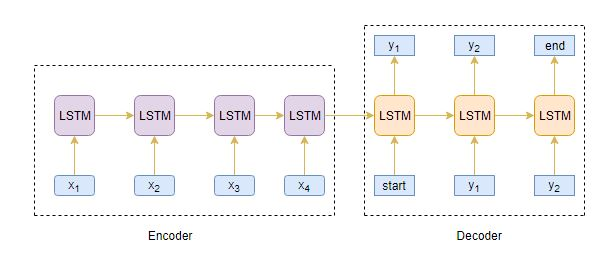
\includegraphics[width=15cm]{img/seq2seq-model.jpg}
\caption{Model slijed-u-slijed arhitekture (seq2seq) (\citet{article3})}
\label{fig:seq2seq-model}
\end{figure}
Dvije glavne komponente seq2seq modela su koder (eng. encoder) i dekoder (eng.decoder).
Koder-dekoder arhitektura se uglavnom koristi za rješavanje slijed-u-slijed (seq2seq) problema gdje su ulazni i izlazni slijed različite duljine.
Ulaz je dugačak niz riječi, a izlaz će biti sažeti (kraći) ulaz.
\begin{figure}[htb]
\centering
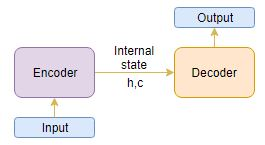
\includegraphics[width=10cm]{img/encoder-decoder-architecture.jpg}
\caption{Model koder-dekoder arhitekture (\citet{article3})}
\label{fig:encoder-decoder}
\end{figure}
Općenito se kao model koder-dekoder arhitekture preferiraju varijante povratne neuronske mreže (eng. recurrent neural networks (RNNs)) kao što su "gated recurrent neural network" (GRU) ili "long short term memory" (LSTM) (\citet{article3}).
Njihova prednost je u tome što su sposobne uhvatiti dugoročne ovisnosti prevladavajući problem nestajanja gradijenta.
Za implementaciju mreže korišten je LSTM model.
\par Koder-dekoder arhitektura se postavlja u dvije faze:
\begin{itemize}
    \item faza treninga
    \item faza zaključivanja
\end{itemize}

\section{Faza treninga}
U fazi treninga prvo se postavljaju koder i dekoder. Nakon toga, model se trenira kako bi ispravno predvidio ciljni (izlazni) slijed koji je zakašnjen za jedan vremenski korak.
Model LSTM kodera prvo čita cijeli ulazni niz gdje se u svakom vremenskom koraku jedna riječ ubacuje u koder.
Model tada obrađuje informacije u svakom vremenskom koraku i hvata kontekstualne informacije prisutne u ulaznom slijedu.
\begin{figure}[htb]
\centering
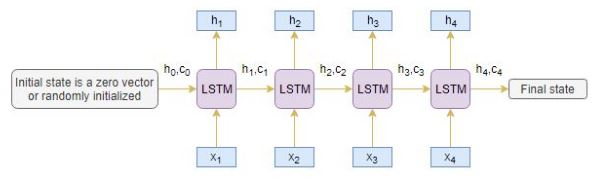
\includegraphics[width=15cm]{img/LSTM-encoder.jpg}
\caption{Model LSTM kodera (\citet{article3})}
\label{fig:LSTM-encoder}
\end{figure}
Skriveno stanje h\textsubscript{i} i stanje ćelije c\textsubscript{i} zadnjeg vremenskog koraka se koriste za inicijalizaciju dekodera.
Dekoder je također LSTM mreža koja čita cijeli ciljni niz riječ po riječ i predviđa upravo taj niz zakašnjen za jedan vremenski korak.
Dakle, dekoder se trenira kako bi predvidio sljedeću riječ izlaznog niza na temelju prethodne riječi.
\begin{figure}[htb]
\centering
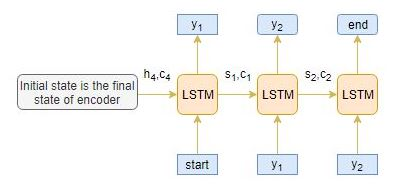
\includegraphics[width=15cm]{img/LSTM-decoder.jpg}
\caption{Model LSTM dekodera (\citet{article3})}
\label{fig:LSTM-decoder}
\end{figure}
Riječi \emph{start} i \emph{end} su posebni tokeni koji se dodaju ciljnom slijedu prije nego što se pošalju u dekoder.
Ciljni slijed je nepoznat za vrijeme dekodiranja testirajućeg slijeda.
Dakle, predviđanje ciljnog slijeda započinjemo tako što prvo pošaljemo token \emph{start} u dekoder.
Token \emph{end} signalizira kraj slijeda.

\section{Faza zaključivanja}
Nakon treniranja model se testira na novim (dosad neviđenim) ulaznim sljedovima za koje ciljani slijed nije poznat.
U tu svrhu postavlja se arhitektura zaključivanja (eng. inference architecture) za dekodiranje testirajućeg slijeda kao što je prikazano na slici ispod.
\begin{figure}[htb]
\centering
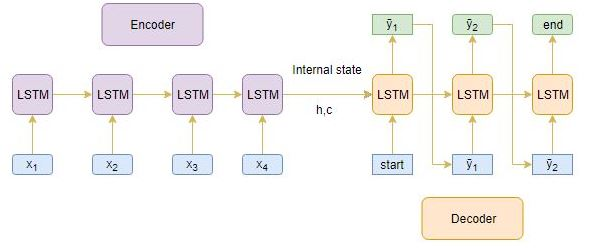
\includegraphics[width=15cm]{img/inference-architecture.jpg}
\caption{Arhitektura zaključivanja (\citet{article3})}
\label{fig:inference-architecture}
\end{figure}
Proces zaključivanja (dekodiranja testirajućeg slijeda) funkcionira ovako (\citet{article3}):
\begin{enumerate}
    \item Kodira se cijeli ulazni slijed i inicijalizira se dekoder unutarnjim stanjima kodera.
    \item Pošalje se \emph{start} token kao ulaz dekoderu.
    \item Pokrene se dekoder za jedan vremenski korak s unutarnjim stanjima.
    \item Izlaz će biti vjerojatnost sljedeće riječi. Riječ s najvećom vjerojatnošću će biti odabrana.
    \item Prosljeđuje se uzorkovana riječ kao ulaz dekoderu u sljedećem vremenskom koraku i ažuriraju se unutarnja stanja trenutnim vremenskim korakom.
    \item Ponavljaju se koraci 3-5 sve dok se ne generira \emph{end} token ili dok se ne dosegne maksimalna duljina ciljanog slijeda.
\end{enumerate}

\section{Ograničenja koder-dekoder arhitekture}
Jedno od glavnih ograničenja s kojima se susreće koder-dekoder arhitektura proizlazi iz činjenice da koder pretvara cijeli ulazni slijed u vektor fiksne duljine i tada dekoder predviđa izlazni slijed (\citet{article3}). To funkcionira samo za kratke sljedove jer dekoder razmatra cijeli ulazni slijed kako bi napravio predviđanje.
Problem dugih ulaznih sljedova je u tome što je koderu teško preslikati (sažeti) dugačke sljedove u vektore fiksne duljine.
Performanse obične koder-dekoder arhitekture naglo padaju kako se povećava duljina ulaznih rečenica.
Ovaj problem koder-dekoder arhitekture se rješava pomoću mehanizma pažnje (eng. attention mechanism).
Mehanizam pažnje pokušava predvidjeti riječ na temelju nekoliko specifičnih dijelova ulaznog slijeda, umjesto razmatranja cijelog ulaznog slijeda.
\subsection{Mehanizam pažnje}
Intuicija iza mehanizma pažnje se može opisati sljedećim pitanjem: \emph{Koliko pažnje moramo posvetiti svakoj pojedinoj riječi ulaznog slijeda za generiranje riječi izlaznog slijeda u trenutku t?}
Dakle, umjesto razmatranja svih riječi ulaznog slijeda, može se povećati značaj pojedinih dijelova ulaznog slijeda čime se dobiva izlazni slijed (sastavljen od najvažnijih dijelova ulaznog slijeda).
Postoje dvije vrste mehanizma pažnje, ovisno o načinu na koji je izveden kontekstualni vektor pažnje:
\begin{itemize}
    \item globalna pažnja
    \item lokalna pažnja
\end{itemize}
\par
Kod globalne pažnje, pažnja se pridaje svim ulaznim pozicijama. Drugim riječima, sva skrivena stanja kodera se uzimaju u obzir za dobivanje kontekstualnog vektora pažnje.
\par
Kod lokalne pažnje, pažnja se pridaje samo nekim ulaznim pozicijama. Samo nekoliko skrivenih stanja kodera se uzimaju u obzir za dobivanje kontekstualnog vektora pažnje.
\par
Za implementaciju mreže korištena je globalna pažnja.
\begin{figure}[htb]
\centering
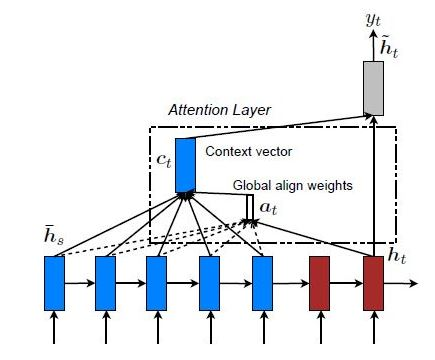
\includegraphics[width=15cm]{img/global-attention.jpg}
\caption{Globalna pažnja (\citet{article3})}
\label{fig:global-attention}
\end{figure}
Mehanizam pažnje radi na sljedeći način (\citet{article3}).
\begin{enumerate}
    \item Koder daje kao izlaz skriveno stanje (h\textsubscript{j}) za svaki vremenski korak j u ulaznom slijedu.
    \item Dekoder daje kao izlaz skriveno stanje (s\textsubscript{i}) za svaki vremenski korak i u ciljnom slijedu.
    \item Računa se vrijednost koja se naziva vrijednost poravnanja (e\textsubscript{ij}) pomoću koje se izvorna riječ poravnava s ciljanom riječi koristeći prikladnu funkciju. Vrijednost poravnanja se računa na temelju skrivenog stanja kodera (h\textsubscript{j}) i skrivenog stanja dekodera (s\textsubscript{i}) koristeći pritom neku od funkcija kao što su skalarni produkt, aditivna ili opća funkcija.
    \item Normaliziraju se vrijednosti poravnanja koristeći softmax funkciju kako bi se dobile težine pažnje (a\textsubscript{ij}).
    \item Računa se linearna suma produkata težina pažnje a\textsubscript{ij} i skrivenih stanja kodera h\textsubscript{j} kako bi se dobio kontekstualni vektor pažnje (C\textsubscript{i}).
    \item Kontekstualni vektor pažnje i skriveno stanje dekodera se u vremenskom koraku i ulančavaju kako bi se dobio skriveni vektor pažnje (S\textsubscript{i}).
    \item Skriveni vektor pažnje S\textsubscript{i} se tada šalje u gusti sloj kako bi se dobio izlaz y\textsubscript{i}.
\end{enumerate}


\section{Opis problema i implementacija}
Cilj vlastite neuronske mreže je sažimanje recenzija iz "Amazon Fine Food reviews" skupa podataka.
Pri tome je ostvareno apstrakcijsko sažimanje teksta koristeći prethodno opisanu koder-dekoder arhitekturu s globalnom pažnjom.
Za implementaciju u Pythonu korištene su programske knjižnice Tensorflow i Keras.
Implementacija globalne pažnje preuzeta je i smještena u datoteku \emph{attention.py} jer Keras nema potporu za rad sa slojem pažnje.
Neke od ostalih knjižnica koje su korištene su numpy, pandas, BeautifulSoup, Tokenizer, nltk, stopwords i slično.
Za potrebe treniranja mreže pročitano je 120 000 redaka iz "Amazon Fine Food reviews" csv baze podataka.
\par
Nakon toga su pročitani podatci obrađeni za potrebe treniranja mreže.
To znači da su odbačeni duplikati, izbačene N/A vrijednosti, proširene kontrakcije, uklonjene kratke riječi, filtrirane samo recenzije i sažetci koji su kraći od prethodno postavljene maksimalne duljine, dodani su \emph{START} i \emph{END} tokeni na početak odnosno kraj svakog sažetka, skup podataka je podijeljen na skup za treniranje i skup za validaciju u omjeru 9:1, pripremljeni su tokenizatori za recenzije i sažetke na temelju obrađenih podataka, podatci su pretvoreni u sljedove prirodnih brojeva te su izbačeni oni reci koji sadrže samo \emph{START} i \emph{END} tokene.
\par
Nakon pripreme podataka za treniranje slijedi stvaranje modela mreže.
Kao što je u prethodnom poglavlju detaljno opisano, korištena je koder-dekoder LSTM arhitektura s globalnom pažnjom.
Za izradu kodera su korištene 3 LSTM mreže složene jedna na drugu.
Dekoder je također LSTM mreža spojena na izlaze kodera. Za spajanje kodera i dekodera korišten je sloj ugradnje.
Sloj pažnje je spojen na izlaze kodera i dekodera.
Na kraju, izlaz iz dekodera se spaja s izlazom iz sloja pažnje te se koristi gusti sloj za konačnu obradu izlaza ovog modela.
\par
Nakon definicije model se trenira na prethodno obrađenom skupu podataka i spremaju se dobivene težine koje se kasnije koriste za postavljanje modela (učitavaju se težine umjesto ponovnog treniranja).


\chapter{Opis postupka vrednovanja mreže}
Prilikom treniranja mreže korištena je rijetka unakrsna kategorična entropija (eng. sparse categorical cross-entropy) kao funkcija gubitka jer ona u letu pretvara sljedove cijelih brojeva u \emph{one-hot} vektore, čime se zaobilaze mogući problemi s memorijom.
Korišten je i koncept ranog zaustavljanja (eng. early stopping) gdje je definirano da će treniranje prestati onda kada se povećaju gubitci prilikom validacije.
Model je treniran na veličini serije (eng. batch size) od 512.
Nakon 10. epohe je došlo do pada performansi (odnosno povećanja gubitaka prilikom validacije), pa je treniranje u tom trenutku prestalo.
\par
Nakon treniranja slijedi proces zaključivanja, dakle proces gdje dekoder sam na temelju ulaza generira sažetak.
Sažetci su relativno kratki i čini se da su pristrani na pozitivnu stranu, jer u većini slučajeva djeluju optimističnije od originalnih recenzija.
Mogući načini za poboljšanje performansi modela su:
\begin{itemize}
    \item Povećanje veličine skupa podataka za treniranje. U tom slučaju bi model trebao biti sposobniji za generalizaciju.
    \item Korištenje dvosmjernih LSTM modela koji su sposobni da uhvate kontekst iz oba smjera i time stvaraju bolji kontekstualni vektor.
    \item Korištenje strategije pretraživanja snopa za dekodiranje ispitnog slijeda umjesto korištenja pohlepnog pristupa (argmax).
    \item Ocjena performansi modela na temelju BLEU rezultata.
    \item Implementacija mreže pokazivača-generatora i mehanizama pokrivanja.
\end{itemize}


\chapter{Zaključak}
Sažimanje teksta je grana strojnog učenja, konkretnije obrade prirodnog jezika, kojoj je cilj stvoriti sažeti prikaz originalnog teksta koji u sebi nosi glavne ideje i najvažnije informacije.
Postoje dva glavna pristupa sažimanju teksta: ekstrakcijsko sažimanje teksta i apstrakcijsko sažimanje teksta.
Ekstrakcijsko sažimanje teksta izvlači rečenice ili ključne izraze iz teksta koji se na kraju spajaju u sažetak. Ne generiraju se novi izrazi niti rečenice. Ovaj način je popularniji zato što je znatno jednostavniji.
Apstrakcijsko sažimanje teksta uključuje parafraziranje i kraćenje dijelova iz teksta. Time nastaju nove rečenice i izrazi. Ovaj način je sličniji ljudskom načinu sažimanja teksta (prepričavanje), ali je znatno složeniji.
Sažimanje teksta se uobičajeno tretira kao nadzirano strojno učenje gdje se budući rezultati predviđaju na temelju pruženih podataka: ulaz i željeni izlaz.
U radu je implementiran programski sustav za sažimanje teksta u Pythonu koji omogućuje oba gore navedena načina sažimanja teksta.
Za ekstrakcijsko sažimanje teksta su korištene programske knjižnice kao što su SpaCy, NLTK, Gensim i Sumy dok je za potrebe apstrakcijskog sažimanja teksta dizajnirana i istrenirana neuronska mreža koja sažima kraće recenzije.
Neuronska mreža stvara relativno kratke sažetke koji su u većini slučajeva optimističniji od originalnog teksta.


\bibliography{literatura}
\bibliographystyle{fer}

\begin{sazetak}
Tema rada je bila proučiti primjenu strojnog učenja u sažimanju teksta. Postoje dva glavna tipa sažimanja teksta: ekstrakcijsko i apstrakcijsko sažimanje teksta.
Ekstrakcijsko sažimanje teksta izvlači rečenice ili ključne izraze iz teksta koji se na kraju spajaju u sažetak, dok apstrakcijsko sažimanje teksta uključuje parafraziranje i kraćenje dijelova iz teksta.
Napravljena je Python aplikacija pomoću TkInter-a koja omogućuje sažimanje teksta na oba načina.
Za ekstrakcijsko sažimanje teksta korištene su neke od poznatih programskih knjižnica u Pythonu kao što su SpaCy, Gensim, NLTK, Sumy i slično, dok je za potrebe apstrakcijskog sažimanja teksta dizajnirana i istrenirana neuronska mreža pomoću programskih biblioteka Tensorflow i Keras.


\kljucnerijeci{Duboko učenje, Obrada prirodnog jezika, Sažimanje teksta, Python}
\end{sazetak}

% TODO: Navedite naslov na engleskom jeziku.
\engtitle{Text Summarization Based on Deep Learning Models}
\begin{abstract}
The topic of the paper was to study the application of machine learning in text summarization. There are two main types of text summarization: extraction and abstraction based text summarization.
Extractive text summarization extracts sentences or key phrases from the text that are then merged into a summary, while abstractive text summarization involves paraphrasing and shortening parts of the text.
A Python application was created using TkInter that allows text to be summarized in both ways.
Some of the well-known program libraries in Python, such as SpaCy, Gensim, NLTK and Sumy were used for extractive text summarization, while a neural network was designed and trained using Tensorflow and Keras libraries for the purpose of abstractive text summarization.

\keywords{Deep learning, Natural language processing, Text summarization, Python}
\end{abstract}


\end{document}
